\section{Estudio Técnico}
 
\subsection{Análisis del Tamaño del Proyecto}

El tamaño del proyecto se estima considerando a la cantidad de bandas en 
que accederán al servicio en un periodo determinado.

Considerando que el horario de funcionamiento es desde las 09:00 horas
a las 24:00 horas y que el arriendo de la sala de ensayo y el estudio
de grabación es por periodos de una hora c/u. Por lo tanto en un día 
será posible atender a:

\begin{table}[h]
    \centering
	\begin{tabular}{|l|l|c|}
		\hline
			\textbf{Sala de ensayo (hrs)}       & 15 \\\hline
			\textbf{Estudio de grabación (hrs)} & 15 \\\hline
			\textbf{Total (hrs)}                & 30 \\\hline
	\end{tabular}
\caption{Horas de funcionamiento de la sala de ensayo y estudios de grabación}
\end{table}
 
% falta decir cual es el espacio que requiere el proyecto no?
% Acá voy a agregarle challa correspondiente a ello:
En el caso más extremo, será posible atender a un máximo de 26 bandas en un
día, por lo que el proyecto requeriría de al menos una sala de grabación, salón
de eventos y una oficina para asuntos administrativos.

Además, se necesita de espacios para almacenar todos los instrumentos y
herramientas necesarias para el funcionamiento normal de los servicios
ofrecidos.

Por último, es recomendable que el espacio físico del local
cuente con espacios suficientes para poder contar con vehículos de transporte
(para los instrumentos, herramientas y personal, según sea necesario).


\subsection{Localización del Proyecto}

\subsubsection{Orientación de la localización}
La localización del proyecto está orientada a seleccionar los factores necesarios 
para maximizar los beneficios del proyecto, principalmente centrados en 
criterios económicos, estratégicos, institucionales y preferencias del equipo.
En la siguiente sección, se explica detalladamente que factores se consideraron
para establecer el estudio de macrolocalización y el estudio de microlocalización,
finalmente se obtuvo la ubicación exacta del proyecto.

\subsubsection{Factores que inciden en la localización de este proyecto}
Los criterios a utilizar para definir la macrolocalización son los siguientes:
\begin{itemize}
	\item Económicos.
	\item Estratégicos.
	\item Institucionales.
	\item Preferencias emocionales.
\end{itemize}

Para determinar en que región de Chile desarrollar el proyecto se han definido
5 factores de localización y a cada uno se le ha otorgado un peso.
Los factores y su clasificación se presentan a continuación en la tabla 5.

\begin{table}[h]
\centering
	\begin{tabular}{|c|c|c|c|}
		\hline
		\textbf{Id} & \textbf{Factor} & 
		\textbf{Clasificación} & \textbf{Peso} \\
		\hline
		1      & Fracción del segmento objetivo  & Económico    & 5 \\
		\hline
		2      & Cantidad de Universidades       & Estratégico  & 3 \\
		\hline
		3      & Cantidad de oferta por región   & Económico    & -6 \\
		\hline
		4      & Cantidad de centros de eventos  & Estratégico  & 4 \\
		\hline
		5      & Preferencia personal del equipo & Preferencias & 3 \\
		\hline
	\end{tabular}
\caption{Factores de localización por región}
\label{tab:macrolocalizacion}
\end{table}
%

A continuación, se presenta una breve justificación de la elección de estos factores.

\begin{enumerate}
	\item \textbf{Fracción del segmento objetivo}: Al definir el mercado objetivo
	se determinó enfocar el servicio al nivel socioeconómico C2 y C3 por lo cual
	es pertinente determinar la distribución regional de este segmento. Como peso se 
	consideró la suma de los porcentajes de los niveles socioeconómicos C2 y C3 con respecto
	al país.
	\item \textbf{Cantidad de Universidades por región:} Las Universidades concentran un gran
	número de bandas emergentes por lo cual, es un factor relevante en el éxito del servicio.
	El peso de este factor corresponde al porcentaje de la cantidad de bandas por región.
	\item \textbf{Competencia por región}: La distribución de salas de ensayo y/o estudios de grabación 
	por región permitirá medir el nivel de competitividad del mercado. El peso de este factor
	corresponde al porcentaje de estudios de grabación y salas de ensayo.
	\item \textbf{Cantidad de centros de eventos por región}: Es un factor estratégico clave para 
	el logro de los objetivos del servicio. El peso de este factor es el porcentaje de centros de eventos
	por región.
	\item \textbf{Preferencia personal del equipo}. el 100\% de preferencia se divide entre las distintas regiones
	preferidas por el equipo para desarrollar el proyecto.
\end{enumerate}

Ahora, para el buen posicionamiento del local, se deben considerar diversos
factores relacionados con el impacto del mismo con el lugar establecido.
De los impactos negativos que se podrían generar está el ruido ambiental, el
cual debe considerarse para evitar problemas con otros agentes de la vecindad.

Además, se consideran importantes los siguientes factores:

\begin{enumerate}
    \item \textbf{Centralidad:} Es importante que el lugar sea de fácil acceso,
    quedando cerca de otros servicios para los clientes, de tal forma que de
    verdad sea conveniente para ellos utilizar los servicios.
    \item \textbf{Espacios abiertos:} Contemplando expansiones futuras y la
    realización de eventos en espacios abiertos, sería muy positivo que le
    proyecto contara con un espacio considerable fuera del inmueble.
    \item \textbf{Tamaño del inmueble:} El proyecto requiere de un tamaño
    mínimo de 400 metros cuadrados. Este espacio considera las salas de
    ensayo, de grabación, sala de reuniones, bodega y espacios administrativos.
    \item \textbf{Calidad y servicios:} El material y arquitectura que posea
    el inmueble definirá cual será la inversión extra que deberá hacerse para
    lograr tener salas con aislación de sonido y/o mantención general del
    inmueble. Además, se consideran todas las características y servicios que
    ya posea la propiedad, como estacionamientos que permitan
    un fácil acceso y espacios para almacenar instrumentos.
    \item \textbf{Precio:} El inmueble debe encontrarse dentro del presupuesto
    del proyecto, siendo ideal minimizar el costo del arriendo del mismo.
\end{enumerate}

\begin{table}[htb!]
\centering
\begin{tabular}{|l|c|}
\hline
\textbf{Criterio}   & \textbf{Peso}\\
\hline
Centralidad         & 5    \\
Espacios abiertos   & 1   \\
Tamaño del inmueble & 4   \\
Calidad y servicios & 3   \\
Precio              & 2   \\
\hline
\end{tabular}
\caption{Peso de cada criterio de evaluación utilizado para la
microlocalización del proyecto}
\label{tab:resumen}
\end{table}
\newpage
\subsubsection{Macrolocalización}
Se han evaluado los factores de macrolocalización en cada región (Ver el anexo para una referencia detallada de los datos) y se ha obtenido
una ponderación total por región la cual determina donde es más
conveniente desarrollar el proyecto. Para normalizar los pesos de cada uno de los factores, se calculó
el porcentaje de aparición del factor con respecto al total nacional en todos los casos.
\begin{table}[!htb!]
\centering
	\begin{tabular}{|c|c|c|c|}
	\hline
	\multicolumn{4}{|c|}{\textbf{I Región}} \\
	\hline
	\textbf{Factor}                              & \textbf{Calificación} & \textbf{Peso} & \textbf{Ponderación} \\
	\hline
	Segmento Objetivo                            & 7,2                    & 5                     & 36 \\
	\hline
	Universidades                                & 4.8                    & 3                     & 14,4\\
	\hline
	Competencia                                  & 0,6                    & -6                    & -3,6 \\
	\hline
	Eventos                                      & 3,3                    & 4                     & 13,2 \\
	\hline
	Preferencia personal                         & 0                      & 3                     & 0 \\
	\hline
	\multicolumn{3}{|c|}{\textbf{Total}}         & \textbf{\blue{60}}\\
	\hline
	\multicolumn{4}{|c|}{\textbf{II Región}} \\
	\hline
	\textbf{Factor}                              & \textbf{Calificación} & \textbf{Peso} & \textbf{Ponderación} \\
	\hline
	Segmento Objetivo                            & 8,8                    & 5                     & 44 \\
	\hline
	Universidades                                & 4                      & 3                     & 12 \\
	\hline
	Competencia                                  & 1,5                    & -6                    & -9 \\
	\hline
	Eventos                                      & 3,9                    & 4                     & 15,6 \\
	\hline
	Preferencia personal                         & 0                      & 3                     & 0 \\
	\hline
	\multicolumn{3}{|c|}{\textbf{Total}}         & \textbf{\blue{62,6}}\\
	\hline
	\multicolumn{4}{|c|}{\textbf{III Región}} \\
	\hline
	\textbf{Factor}                              & \textbf{Calificación} & \textbf{Peso } & \textbf{Ponderación} \\
	\hline
	Segmento Objetivo                            & 3,1                    & 5                     & 15,5 \\
	\hline
	Universidades                                & 3,2                    & 3                     & 9,6 \\
	\hline
	Competencia                                  & 0                      & -6                    & 0 \\
	\hline
	Eventos                                      & 1.5                    & 4                     & 6 \\
	\hline
	\multicolumn{3}{|c|}{\textbf{Total}} &\textbf{\blue{31,1}}\\
	\hline
	\multicolumn{4}{|c|}{\textbf{IV Región}} \\
	\hline
	\textbf{Factor}                                        & \textbf{Calificación}           & \textbf{Peso} & \textbf{Ponderación} \\
	\hline
	Segmento Objetivo                                      & 6.4                     & 5                     & 32 \\
	\hline
	Universidades                                          & 7,3                     & 3                     & 21,6\\
	\hline
	Competencia                                            & 1,5                     & -6                    & -9 \\
	\hline
	Eventos                                                & 4,5                     & 4                     & 18 \\
	\hline
	Preferencia personal                                   & 0                       & 3                     & 0 \\
	\hline
	\multicolumn{3}{|c|}{\textbf{Total}}                   & \textbf{\blue{62,6}}\\
	\hline
	\end{tabular}
\end{table}
\newpage
\begin{table}[htb!]
\centering
	\begin{tabular}{|c|c|c|c|}
	\hline
	\multicolumn{4}{|c|}{\textbf{V Región}} \\
	\hline
	\textbf{Factor}                                        & \textbf{Calificación}           & \textbf{Peso} & \textbf{Ponderación} \\
	\hline
	Segmento Objetivo                                      & 22.7                    & 5                     & 113,5 \\
	\hline
	Universidades                                          & 9,6                     & 3                     & 28,8 \\
	\hline
	Competencia                                            & 4,8                     & -6                    & -28,8 \\
	\hline
	Eventos                                                & 13,6                    & 4                     & 54,4 \\
	\hline
	Preferencia personal                                   & 60                      & 3                     & 180 \\
	\hline
	\multicolumn{3}{|c|}{\textbf{Total}}                   & \textbf{\blue{347,9}}\\
	\hline
	\multicolumn{4}{|c|}{\textbf{VI Región}} \\
	\hline
	\textbf{Factor}                                        & \textbf{Calificación}           & \textbf{Peso} & \textbf{Ponderación} \\
	\hline
	Segmento Objetivo                                      & 7.2                     & 5                     & 36 \\
	\hline
	Universidades                                          & 4,8                     & 3                     & 14,4 \\
	\hline
	Competencia                                            & 1,5                     & -6                    & -9 \\
	\hline
	Eventos                                                & 2,4                     & 4                     & 9,6 \\
	\hline
	Preferencia personal                                   & 0                       & 3                     & 0 \\
	\hline
	\multicolumn{3}{|c|}{\textbf{Total}}                   & \textbf{\blue{51}}\\
	\hline

	\multicolumn{4}{|c|}{\textbf{VII Región}} \\
	\hline
	\textbf{Factor}                                        & \textbf{Calificación}           & \textbf{Peso} & \textbf{Ponderación} \\
	\hline
	Segmento Objetivo                                      & 7.1                     & 5                     & 35.5 \\
	\hline
	Universidades                                          & 6,4                     & 3                     & 19,2 \\
	\hline
	Competencia                                            & 0.6                     & -6                    & -3.6 \\
	\hline
	Eventos                                                & 2,4                     & 4                     & 9,6 \\
	\hline
	Preferencia personal                                   & 0                       & 3                     & 0 \\
	\hline
	\multicolumn{3}{|c|}{\textbf{Total}}                   & \textbf{\blue{60,7}}\\
	\hline

	\multicolumn{4}{|c|}{\textbf{VIII Región}} \\
	\hline
	\textbf{Factor}                                        & \textbf{Calificación}           & \textbf{Peso} & \textbf{Ponderación} \\
	\hline
	Segmento Objetivo                                      & 19.4                    & 5                     & 97 \\
	\hline
	Universidades                                          & 11,2                    & 3                     & 33,6 \\
	\hline
	Competencia                                            & 0.3                     & -6                    & -1.8 \\
	\hline
	Eventos                                                & 9,3                     & 4                     & 37,2 \\
	\hline
	Preferencia personal                                   & 40                      & 3                     & 90 \\
	\hline
	\multicolumn{3}{|c|}{\textbf{Total}}                   & \textbf{\blue{286}}\\
	\hline
	\multicolumn{4}{|c|}{\textbf{IX Región}} \\
	\hline
	\textbf{Factor}                                        & \textbf{Calificación}           & \textbf{Peso} & \textbf{Ponderación} \\
	\hline
	Segmento Objetivo                                      & 7.3                     & 5                     & 36.5 \\
	\hline
	Universidades                                          & 6,4                     & 3                     & 19,2 \\
	\hline
	Competencia                                            & 0                       & -6                    & 0 \\
	\hline
	Eventos                                                & 3,9                     & 4                     & 15,6 \\
	\hline
	Preferencia personal                                   & 0                       & 3                     & 0 \\
	\hline
	\multicolumn{3}{|c|}{\textbf{Total}}                   & \textbf{\blue{71,3}}\\
	\hline
\end{tabular}
\end{table}
\newpage
\begin{table}[htb!]
\centering
	\begin{tabular}{|c|c|c|c|}
	\hline
	\multicolumn{4}{|c|}{\textbf{X Región}} \\
	\hline
	\textbf{Factor}                                        & \textbf{Calificación}           & \textbf{Peso} & \textbf{Ponderación} \\
	\hline
	Segmento Objetivo                                      & 8.8                     & 5                     & 44 \\
	\hline
	Universidades                                          & 4,8                     & 3                     & 14,4 \\
	\hline
	Competencia                                            & 0                       & -6                    & 0 \\
	\hline
	Eventos                                                & 5,4                     & 4                     & 21,6 \\
	\hline
	Preferencia personal                                   & 0                       & 3                     & 0 \\
	\hline
	\multicolumn{3}{|c|}{\textbf{Total}}                   & \textbf{\blue{80}}\\
	\hline
	\multicolumn{4}{|c|}{\textbf{XI Región}} \\
	\hline
	\textbf{Factor}                                        & \textbf{Calificación}           & \textbf{Peso} & \textbf{Ponderación} \\
	\hline
	Segmento Objetivo                                      & 0.9                     & 5                     & 4,5 \\
	\hline
	Universidades                                          & 2,4                     & 3                     & 7,2 \\
	\hline
	Competencia                                            & 0                       & -6                    & 0 \\
	\hline
	Eventos                                                & 0,6                     & 4                     & 2,4 \\
	\hline
	Preferencia personal                                   & 0                       & 3                     & 0 \\
	\hline
	\multicolumn{3}{|c|}{\textbf{Total}}                   & \textbf{\blue{14,1}}\\
	\hline

	\hline
	\multicolumn{4}{|c|}{\textbf{XII Región}} \\
	\hline
	\textbf{Factor}                                        & \textbf{Calificación}           & \textbf{Peso} & \textbf{Ponderación} \\
	\hline
	Segmento Objetivo                                      & 2.4                     & 5                     & 12 \\
	\hline
	Universidades                                          & 2,4                     & 3                     & 7,2 \\
	\hline
	Competencia                                            & 0                       & -6                    & 0 \\
	\hline
	Eventos                                                & 0,9                     & 4                     & 3,6 \\
	\hline
	Preferencia personal                                   & 0                       & 3                     & 0 \\
	\hline
	\multicolumn{3}{|c|}{\textbf{Total}}                   & \textbf{\blue{22,8}}\\
	\hline

	\hline
	\multicolumn{4}{|c|}{\textbf{Región Metropolitana}} \\
	\hline
	\textbf{Factor}                                        & \textbf{Calificación}           & \textbf{Peso} & \textbf{Ponderación} \\
	\hline
	Segmento Objetivo                                      & 97.6                    & 5                     & 488 \\
	\hline
	Universidades                                          & 32,2                    & 3                     & 96,6 \\
	\hline
	Competencia                                            & 88.9                    & -6                    & -533.4 \\
	\hline
	Eventos                                                & 47,5                    & 4                     & 190 \\
	\hline
	Preferencia personal                                   & 0                       & 3                     & 0 \\
	\hline
	\multicolumn{3}{|c|}{\textbf{Total}} &\textbf{\blue{241,2}}\\
	\hline
\end{tabular}
\caption{Factores de localización por Región. Fuente: Elaboración Propia.}
\label{tab:resultados}
\end{table}
El proyecto se realizará en la \textbf{V Región} ya que es la región que presenta en mayor proporción los factores
considerados alcanzando una puntuación de \textbf{347,9 puntos}.
\newpage
\newpage
\subsubsection{Microlocalización}
Considerando los criterios nombrados anteriormente, se evaluaron los siguientes inmuebles dentro de Viña del Mar:
\begin{enumerate}
%Código 698840
%Contacto   CRISTIAN DIAZ ARAVENA
%Dirección  Av. San Martin 616 (entre 7 y 8 Norte)
%Teléfono(s)     (9) 9927 8890 / (032) 319 8610
%E-mail INFO@RENTAMAR.CL
%http://www.portalinmobiliario.com/propiedades/fichas.asp?PropID=698840&Pag=1&Ant=&Sig=2&TId=1&MoID=2&OId=2,4&IdCom=72&S1=400&P2=1
    \item Casona en calle Alvarez 699, cerca de la parroquia:\\  Estacionamientos, despensa, hall de acceso, 5 baños y 10 dormitorios
% http://www.portalinmobiliario.com/propiedades/fichas.asp?PropID=1025897&Pag=1&Ant=2&Sig=4&TId=1&MoID=2&OId=2,4&IdCom=72&S1=400&P2=1
    \item Casa en Cerro Castillo:\\
    4 Dormitorios y Baños, 1 Suite.
%http://www.portalinmobiliario.com/propiedades/fichas.asp?PropID=1051991&Pag=1&Ant=5&Sig=7&TId=1&MoID=2&OId=2,4&IdCom=72&S1=400&P2=1
    \item Casa en 5 Norte:\\ Estacionamiento 2 vehículos, garage, patio trasero
    y antejardin,  10 dormitorios y baños.
% http://www.portalinmobiliario.com/propiedades/fichas.asp?PropID=856884&Pag=1&Ant=11&Sig=13&TId=1&MoID=2&OId=2,4&IdCom=72&S1=400&P2=1
    \item Casona cerca del centro:\\
    19 dormitorios, 7 suites, 13 baños.
% http://www.portalinmobiliario.com/propiedades/fichas.asp?PropID=1033619&Pag=1&Ant=12&Sig=14&TId=1&MoID=2&OId=2,4&IdCom=72&S1=400&P2=1
    \item Casa al lado de la Quinta Vergara:\\
    3 pisos, hall, recepción, 7 salas, 5 oficinas, 2 salas exteriores, 7 baños,
    cocina, repostero y alarma.
% \url{http://www.adoos.cl/postx/ded95cd8540e9fe641db923cf15ceb8b/oficinas_comerciales_400_m2_calle_prat_sector}
    %\item Oficina comercial Calle Prat, Valparaíso:   \\
%\url{http://www.adoos.cl/postx/f2a0250f58ef0f0831f0d334a7133ab8/arriendo_local_comercial_centro_de_viaa_del_mar}
    \item Local Comercial Centro de Viña:     \\
    3 plantas, oficinas y bodefas, 4 baños, cocina y comedor. 
%\{http://www.adoos.cl/post/19994939/arriendo_oficinas_comercial_en_pleno_sector}
    %\item Oficina Calle Esmeralda, Valparaíso:  \\
\end{enumerate}

\begin{table}[htb!]
\centering
\begin{tabular}{|l|c|c|c|c|c|}
\hline
\textbf{Inmueble} & \textbf{Sector}       & \textbf{Construido} ($m^2$) & \textbf{Terreno} ($m^2$) & \textbf{Arriendo} (\$) \\ % & \textbf{Extras}\\
\hline
1                 & Parroquia-Centro      & 400                         & 825                      & 1.000.000 \\%               & Estacionamientos, despensa, hall de acceso, 5 baños y 10 dormitorios \\
2                 & Cerro Castillo        & 500                         & 2000                     & 1.200.000 \\
3                 & Libertad              & 700                         & 850                      & 1.500.000 \\%               & Estacionamiento 2 vehículos, garage, patio trasero y antejardin,  10 dormitorios y baños \\
4                 & Centro                & 600                         & 420                      & 2.500.000 \\
5                 & Centro-Quinta Vergara & 700                         & 680                      & 3.354.822 \\
%                 & Centro Comercial      & 400                         & -                        & 1.420.000 \\%               & \\
6                 & Centro Comercial      & 400                         & -                        & 2.759.584 \\%               & \\
%                 & Centro Comercial      &                             & -                        & 692.555   \\%               & \\
\hline
\end{tabular}
\caption{Inmuebles escrutados en Viña del Mar.}
\label{tab:direcciones}
\end{table}


\begin{table}[htb!]
\centering
\begin{tabular}{|l|c|c|c|c|c|c|c|}
\hline
\textbf{Inmueble} & \textbf{Centralidad}   & \textbf{Espacios}  &
\textbf{Tamaño} & \textbf{Calidad} & \textbf{Precio} & \textbf{Total Ponderado}\\
\hline
% ponderacion  5  1   4    3    5
\textbf{1}   & 4& 2 & 2  & 5 &  5  &  \textbf{70} \\%20 + 2 + 8 +  15 + 25 =
\textbf{2}   & 2& 5 & 3  & 1 &  5  & 55\\  %10 + 5 + 12 + 3 + 25 = 
\textbf{3}   & 3& 2 & 5  & 4 &  4  & 69\\ %15 + 2 + 20 + 12 + 20 =
\textbf{4}   & 5& 1 & 4  & 1 &  2  & 55\\  %25 + 1 + 16 + 3 + 10 = 
\textbf{5}   & 4& 2 & 5  & 2 &  1  & 53\\  %20 + 2 + 20 + 6 + 5  = 
\textbf{6}   & 5& 0 & 2  & 3 &  2  & 52\\  %25 + 0 + 8  + 9 + 10 = 
\hline
\end{tabular}
\caption{Inmuebles escrutados en Viña del Mar.}
\label{tab:direcciones}
\end{table}

\subsubsection{Decisión de localización}

Considerando los factores de localización ya mencionados se ha decidido localizar el proyecto en 
la V Región, específicamente en calle Alvarez 699, justo en la zona central de Viña del Mar.

Las imágenes del lugar se pueden encontrar en la sección del \textbf{Layout}.

% Javier y Cristian

\subsection{Ingeniería del Proyecto}

%Aspectos Generales
%
%Debe determinar la funcion de produccion optima para la utilizacion eficiente y eficaz
%	de los recursos disponibles para la produccion del bien o servicio deseado.
%La ingenieria de proyectos tiene la mayor incidencia sobre la estimacion de los costos
%	de inversion y de operacion del proyecto.
%Necesariamente debe incluirse en los anexos el respaldo de la informacion de precios
%	y costos de los equipos y otros.


% Cristian
\subsubsection{Selección del Proceso Productivo}

El funcionamiento de \emph{Music Labs} está determinado por la realización
de asesorías y prestaciones de servicios a bandas emergentes de la quinta región.

El proceso productivo será realizado utilizando parámetros enfocados
para el desarrollo de actividades relacionadas con asesorías y prestaciones
de servicios. Es importante notar que dentro de los clientes, en este caso,
las bandas emergentes, no son iguales, por lo tanto se posee una gran
flexibilidad y variedad entre los distintos trabajos con cada banda.

{ \bf Orientación}
% al producto
%	estandarizado
%	volumenes grandes
%	fabricacion continua
%	lineas continuas
% al proceso
%	especificos
%	solo a pedido
%	numero reducido
%	organizacion segun proceso
% intermedia
%	multiples productos
%	pedidos de lotes medianos
%	lotes estandarizados
%	ensamblado en linea
%	proceso adaptado al producto

La orientación estará determinada por el proceso en sí, en el cual
los servicios ofrecidos se realizarán mediante a los tipos de asesorías
que se deban entregar (como una especie de pedidos), los cuales
tendrán distintos grados de especificaciones, lo que asegurará
la diferenciación de las solicitudes de cada cliente.

% Principales transformaciones
%	informativas como en telecomunicaciones
%	de intercambio como venta al menudeo
%	fisicas como en la manufactura
%	de ubicacion como en el transporte
%	de almacenamiento como en las bodegas

{ \bf Sistema productivo}
% procesos continuos,
%	en el cual los productos pasan a traves de los procesos directamente comunicados en forma
%	continua enlazandose materia prima y productos terminados.
%	ej: productos como gases, liquidos, celulosa, quimicos.
% flow-shop,
%	Similar a continuo, pero orientado a producto en lineas exclusivas, en el cual continuas
%	unidades de salida siguen una misma secuencia de operaciones, involucrando lineas de
%	produccion.
% job-shop 
%	orientado a trabajos tipo taller, en el cual los productos siguen diferentes trayectorias
%	y secuencias a traves de los procesos y maquinas. Maquinas agrupadas en funciones.

El Sistema Productivo va a corresponder al estilo \emph{Job-Shop}, ya que existen
muchas diferencias entre los servicios que se les puedan brindar a las bandas, ya
que las solicitudes dependerán de distintos factores como, tamaño de la banda, estilo
musical, estado actual, etc.

{ \bf Elementos del sistema}

Se señalan a continuación algunos elementos necesarios
para el correcto funcionamiento de \emph{Music Labs}.

\begin{itemize}
	\item \textbf{Oficina de asesoría}

		La oficina será el lugar físico principal para realizar toda la administración
		de \emph{Music Labs}, siendo además la oficina que tendrá los espacios necesarios
		para poder analizar los nuevos clientes, y poder determinar los planes de acción
		por cada cliente.
	\item \textbf{Sala de ensayo}

		La sala de ensayo estará ubicada al lado de la \emph{Oficina de asesoría}
		en el mejor de los casos. Estará equipada con instrumentos de última tecnología
		acompañado de elementos tecnológicos que ayuden al ensayo de las bandas
		clientes de \emph{Music Labs}.
		La sala de ensayo tendrá un espacio principal para poder administrar su uso,
		pudiendo así solicitar información, o realizar reservas de acuerdo al programa
		de cada cliente.
	\item \textbf{Sala de grabación}

		La sala de grabación estará ubicada al lado de la \emph{Oficina de asesoría}
		en el mejor de los casos. Estará equipada con elementos tecnológicos de última
		generación, para poder ofrecer un servicio de primera categoría a la hora
		de hacer grabaciones en los distintos estilos musicales que existen hoy en día.
		La sala de grabación tendrá un espacio principal para poder administrar su uso,
		pudiendo así solicitar información, o realizar reservas de acuerdo al programa
		de cada cliente.
	\item \textbf{Sala de eventos}

		La sala de eventos estará ubicada cercano  a la \emph{Oficina de asesoría}
		o en un lugar céntrico, lo que servirá para atraer al público correspondiente
		a la hora de poder realizar presentaciones con las nuevas bandas emergentes
		que han contratado el servicio de \emph{Music Labs}.
		La presente sala tendrá un enfoque social, por lo cual muchos detalles
		de implementación serán determinados una vez puesto en marcha el proyecto
		ya que se debe adecuar a las necesidades y gustos del publico de los clientes
		de \emph{Music Labs}.
	\item \textbf{Página web}

		Hoy en día, si una empresa o proyecto, no está en la web, se puede decir
		que el proyecto no existe a los ojos del mundo, por lo que siendo un medio
		de comunicación masivo, es necesario tener un portal, con no sólo información
		de \emph{Music Labs}, si no también con un sistema completo para poder
		realizar la asesoría de bandas en forma digital, brindando la oportunidad
		de comunicarse con profesionales de \emph{Music Labs} mediante correo
		electrónico, aparte de ofrecer cotizaciones online, o centros de ayuda.
	\item \textbf{Asesores (Managers)}

		Se contará con un equipo de asesores profesionales, los cuales
		tendrán como objetivo principal, poder guiar a una banda emergente
		en su camino a la fama, brindándole consejos a la hora de ir evolucionando,
		y entregando todo su apoyo cuando corresponda en ciertas actividades
		de un toque administrativo, con terceros que quieran relacionarse con
		clientes de \emph{Music Labs}.
	\item \textbf{Asesores Técnicos}
		
		Se contará con un equipo de asesores técnicos tanto en la Sala de Ensayo
		como en la Sala de Grabación, los cuales serán los responsables de poder
		aconsejar y/o enseñar a la banda emergente algunas técnicas y formas
		para poder crear la música de la mejor forma posible.
	\item \textbf{Asesores Musicales}
		
		Se contará con un equipo de asesores musicales tanto en la Sala de Ensayo
		como en la Sala de Grabación, los cuales serán los responsables de poder
		aconsejar y/o enseñar a la banda emergente sobre metodologías musicales
		para poder crear la música y guiarlos de acuerdo a las raíces de cada
		estilo musical, refinando, la interpretación y forma de componer.

	\item \textbf{Asesores Web}
	
		Se contará con un equipo de asesores web para poder responsabilizarse
		en cualquier aspecto relacionado a la web 2.0, ya sea el posicionamiento
		web en las redes sociales como en otros lugares de internet, siendo
		la idea central poder guiar a la banda emergente en el mundo digital.

\end{itemize}

{\bf Modo de funcionamiento}

\begin{itemize}
	\item \textbf{Selección de servicios}

		Por medio de la página web, contacto telefónico o de
		una forma presencial se podrá acceder a la contratación
		de alguno de los servicios que ofrece \emph{Music Labs}.

		Primero que todo se deberá seleccionar a que tipo de servicio
		se accederá, si es un servicio completo, sólo el arriendo
		de la sala de ensayo, la grabación de un disco, etc.

		Luego de acuerdo al tipo de la banda que desea contratar
		el servicio, se evaluará dicho cliente, para determinar
		sus necesidades y acciones a futuro.

		Tomando en cuenta todos los factores anteriores, se podrá
		determinar el tipo de servicio y planificación del actuar
		de \emph{Music Labs} con su nuevo cliente.
	\item \textbf{Proceso de evaluación}

		El Proceso de evaluación de cada banda será aplicable a grupos
		de personas que tengan una banda, y posean los instrumentos
		determinados~\footnote{También se prestarán instrumentos en caso de ser necesario, lo cual tendrá un costo extra}.

		Esta etapa consistirá en un conjunto de entrevistas de variados
		aspectos a la banda, como pruebas musicales, evaluación
		del material que tengan a la fecha, estilo musical, etc.

		Cabe señalar que el numero de preguntas o entrevistas, dependerá
		de cada banda, ya que se tiene clara la diferenciación entre
		bandas pequeñas a bandas con muchas variaciones instrumentales.

		Luego de haber realizado este proceso, se procederá
		a realizar una evaluación de la banda, para determinar
		como será la relación entre los servicios solicitados y la banda
		viendo factores, de que si es una banda innovadora,
		o si existe una alta oferta en bandas del mismo estilo musical~\footnote{Los detalles
		de innovación, se realizarán con un catastro actualizado de las bandas de la zona}.
				
	\item \textbf{Propuestas}

		Se realizarán cuatro sub-fases de la propuesta realizada, las cuales
		están determinadas por los distintos aspectos de los servicios
		ofrecidos por \emph{Music Labs}.

	 \begin{itemize}
	 	\item \textbf{Propuesta técnica}
	
			Se presentará un documento con los aspectos técnicos de la propuesta,
			los cuales tendrán información acotada sólo al funcionamiento musical
			de la banda, como balances de sonidos, tonalidades de instrumentos,
			etc.
		\item \textbf{Propuesta artística}
			
			Se presentará un documento con los aspectos artísticos de la propuesta,
			los cuales tendrán información acotada sólo al aporte cultural de la banda
			el cual podrá contener una crítica al desplantes de la banda, manejo
			del escenario, interpretación, etc.
		\item \textbf{Propuesta social}
			
			Se presentará un documento con los aspectos sociales de la propuesta,
			los cuales tendrán información acotada sólo al aporte a la sociedad
			de la banda, el cual podrá contener un análisis acompañado
			con encuestas a un determinado conjunto de personas, respecto a
			características como, estilo musical, la posibilidad de asistir
			a eventos de el estilo de musica, etc~\footnote{Las entrevistas se realizarán en conjuntos de personas
			que se sepa con anterioridad que tienen  agrado por el estilo musical, pues si no, no tendría sentido.}.

		\item \textbf{Propuesta Web}

			Se presentará un documento con los aspectos relacionados con redes
			sociales y web 2.0 que podrán ser de utilidad para la banda
			los cuales señalaran sitios en los cuales les convendrá
			difundir la música, modo de uso de las redes sociales,
			campañas virales de promoción, etc.

		\item \textbf{Propuesta de imagen}
				
			Se presentará un documento con los aspectos de imagen de la propuesta,
			los cuales tendrán información acotada sólo a la apariencia de la banda
			en los distintos espectáculos, videos clip, etc.
			Es importante señalar que no se criticará este aspecto para que todas
			las bandas cumplan con un patrón, si no mas bien es dar un consejo
			a la hora de demostrar las emociones y contenido musical, con la imagen
			que representa la banda emergente.
	 \end{itemize}
	\item \textbf{Realización propuesta asesoría}

		Luego de haber realizado la propuesta anteriormente descrita
		se procederá a realizar una planificación de asesoría,
		lo cual será como un plan de trabajo para con la banda emergente
		a manos de \emph{Music Labs}.

		Al tener dicha planificación, y obteniendo la respuesta afirmativa
		del cliente, la asesoría comenzará.

	\item \textbf{Supervisión de trabajo}

		Al momento de encontrarse en proceso la asesoría a los clientes
		existirá un mecanismo directo de supervisión a cada procedimiento,
		pues es esencial para poder ir re-evaluando la situación en la
		cual la banda se encuentra, para poder ir mitigando riesgos
		o corrigiendo algunas características de la asesoría.
	\item \textbf{Asesoría periódica}

		Existirán instancias luego de una cierta cantidad de tiempo
		que permitirán ir marcando los hitos en cada asesoría,
		los cuales no serán una supervisión constante, sino mas
		bien las actividades determinadas para verificar el plan
		de trabajo y poder hacer reajustes con respecto a tiempo
		de ejecución de algún elemento de la planificación
		original.

		Los hitos serán realizados por un comité de \emph{Music Labs}
		más la banda misma, para a través de una reunión informal
		se traten los problemas surgidos y exista una retroalimentación
		positiva al momento del desarrollo de los servicios.

% TO DO
%\red{- Hay varios puntos descritos anteriormente que corresponden a la
%descripción del producto, más que del 
%proceso productivo.}

\end{itemize}
\newpage
\begin{figure}[h!t]
   \centering
  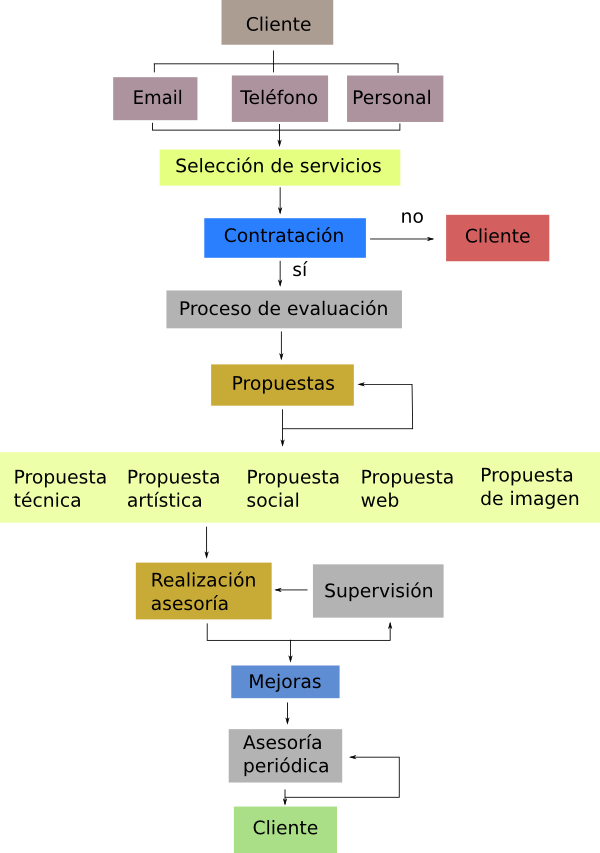
\includegraphics[width=0.9\textwidth]{img/flujo_procesos.png}
   \caption{Diagrama de flujos de proceso}
   \label{fig:flujoprocesos}
\end{figure}
\newpage
% Javier
\subsubsection{Selección de Equipos}
Para el funcionamiento del proyecto serán necesario
los siguientes equipos.

\textbf{Equipos de Oficina}

\begin{itemize}
	\item \textbf{Switch}

		Este dispositivo de Hardware se utiliza para
		permitir que los computadores utilizados en la sala
		de ensayo y estudio de grabación tengan conexión a
		Internet.

	\item \textbf{Computador}

		Servirá para todo el trabajo de
		escritorio relacionado con el servicio brindado.
		No requiere componentes específicos. Es un computador
		distinto al utilizado en la etapa de grabación y
		ensayo. El sistema operativo está incluido en el valor
		del computador.

	\item \textbf{Licencias de Software}

		Se utilizará software de ofimática, 
		además del sistema operativo básico. Se utilizará
		el software que provee Windows. 

	\item \textbf{Impresora}
		Requerida para tareas de oficina.

	\item \textbf{Teléfono}

		Permite la comunicación con los usuarios
		y proveedores para la eventual adquisición de 
		equipos.

	\item \textbf{Mueblería}

		Se incluye un escritorio y dos estantes
		de pared para la ubicación de todo lo
		relacionado con la papelería de la secretaría.
\end{itemize}
	

\textbf{Equipos Sala de Ensayo}
\begin{itemize}
	\item \textbf{Batería}: Se considera una batería completa para el uso
         de las bandas que requieran ensayar.
	\item \textbf{Bajo}: Se considera un bajo electrico para el uso
         de las bandas que requieran ensayar.
	\item \textbf{Guitarras}: Se consideran 3 guitarras. Una guitarra
	      específica para el músico que es primera guitarra. Una
	      segunda guitarra para el guitarrista rítmico. Finalmente
	      considera una guitarra electroacústica.
	\item \textbf{Teclado}: Se considera un teclado electrónico para
         el uso de las bandas que requieran  ensayar.
	\item \textbf{Amplificadores}: Se consideran dos amplificadores de guitarra
	      y uno de bajo.
	\item \textbf{Pedestales de soporte para micrófonos}: Utilizados a favor
         de los intérpretes de cada banda.
	\item \textbf{Micrófonos}: Que se utilizarán para amplificar
	      la voz del vocalista y los integrantes de la banda
	      que hagan coros.
	\item \textbf{Micrófonos batería}: La batería requiere un 
	      set de micrófonos específicos, que sean capaces
	      de amplificar adecuadamente las distintas 
	      frecuencias que ésta emite.
	\item \textbf{Mesa Multipista}: Se requiere un Mixer con 
	      alrededor de 20 canales disponibles. Este equipo
	      recibe las señales enviadas por los micrófonos y amplificadores
	      de instrumentos y luego es capaz de amplificar
	      a través de las cajas acústicas que se detallan a 
	      continuación.
	\item \textbf{Cajas acústicas}: Estas son las encargadas de emitir
	      el sonido que proviene, ya procesado, desde la Mesa
	      Multipista, para que los músicos puedan oir los sonidos que
	      sus instrumentos y voces producen.
	\item \textbf{Cables}: Se requieren cables especialmente diseñados
	      para instrumentos, en este caso para guitarra, bajo
	      y teclado. Las cajas acústicas requieren cable
	      de parlante con conexiones de tipo \textit{speakon}
	      para mayor calidad de sonido. Para los distintos
	      tipos de micrófono se requiere cable de micrófono
	      con conectores XLR-3 macho-hembra.
	\item \textbf{Atriles de instrumentos}: Se considera atriles de soporte
	      para guitarra, bajo y teclado. Este tipo de atril se utiliza
	      para mantener de pie los instrumentos cuando no se están
	      utilizando, salvo el caso del teclado que requiere atril
	      en todo momento.
	\item \textbf{Multipar}: Es un dispositivo que se encarga de encaminar 
	      las distintas señales de audio desde la sala de ensayo
	      a la Mesa de sonido. Contiene una serie de conexiones XLR-3
	      hembra que recibe conectores XLR-3 macho provenientes
	      de los micrófonos y amplificadores de la sala. A través
	      del cableado multipar lleva las señales hacia la mesa de
	      sonido para ser procesado y enviado a través de las cajas
	      acústicas de la sala.
	\item \textbf{Mesa de soporte}: Mesa encargada de sostener la Mesa Multipista.
\end{itemize}

	
\textbf{Equipos de Grabación}
\begin{itemize}
	\item \textbf{Interfaz de Audio}: Dispositivo que permite la adquisición de
	      sonido desde las fuentes de emisión, es decir micrófonos
	      amplificadores, etc. Luego de la captura se procesa y se envía
	      al computador, usando la tarjeta de sonido como entrada, para
	      que se encargue de la grabación.
	\item \textbf{Monitor}: Equipo encargado de reproducir lo que previamente
	      se grabó y procesó. Tiene por finalidad ``monitorear''
	      el avance en el proceso de grabación.
	\item \textbf{Audífonos profesionales}: Dispositivos encargados de 
	      reproducir la base musical que guiará a los músicos 
	      en el proceso de grabación. A través de los audífonos
	      también es posible el envío del metrónomo que dará
	      el tempo de la canción a los encargados de la base rítmica
	      de la canción, que en este caso corresponde al baterista
	      y bajista.
	\item \textbf{Ecualizador Gráfico}: Dispositivo encargado de modificar
	      la señal recibida de los equipos de adquisición de sonido. Este
	      equipo podrá variar las frecuencias bajas, medias y altas obtenidas
	      en el proceso de emisión de sonido.
	\item \textbf{Micrófonos especializados}: Para obtener una grabación de 
	      calidad, se requiere micrófonos técnicamente adaptados para eso.
	      Por esta razón, se requieren dispositivos de captura para los 
	      amplificadores de guitarra, dos micrófonos para bombo y amplificador
	      de bajo y un set de micrófonos para batería. Todos estos equipos
	      tienen características mejoradas que permiten mayor fidelidad de sonido
	      comparado con los micrófonos utilizados en la sala de ensayo. Para
	      la voz se requiere un micrófono de membrana dual y que sea de tipo
	      condensador. Este micrófono requiere un antipop para eliminar
	      ruidos molestos producidos por la respiración del vocalista y por
	      la pronunciación de algunas letras.
	\item \textbf{Cableado para micrófonos}: Se considerarán variados cables blindados
         y de fibra, de 6 metros aproximadamente para el uso de amplificadores.
	\item \textbf{Pedestales de soporte para micrófonos}: Utilizados a favor
         de los intérpretes de cada banda.
	\item \textbf{Computador}: Debe contar con capacidad de almacenamiento alta para 
	      guardar las grabaciones realizadas, considerando el alto peso
	      de los archivos generados por el software de grabación. El computador
	      debe estar equipado con una tarjeta de sonido diseñada específicamente
	      para la labor de adquisición de datos desde la interfaz. Se requiere
	      software especializado en grabación.
	\item \textbf{Mesa de soporte}: Esta debe ser capaz de sostener los
	      distintos equipos detallados anteriormente.
\end{itemize}

\textbf{Equipos de Sala de Eventos}
\begin{itemize}
	\item \textbf{Amplificadores}: Se consideran dos amplificadores de guitarra
	      y uno de bajo.
	\item \textbf{Pedestales de soporte para micrófonos}: Utilizados a favor
         de los intérpretes de cada banda.
	\item \textbf{Micrófonos}: Que se utilizarán para amplificar
	      la voz del vocalista y los integrantes de la banda
	      que hagan coros.
	\item \textbf{Micrófonos batería}: La batería requiere un 
	      set de micrófonos específicos, que sean capaces
	      de amplificar adecuadamente las distintas 
	      frecuencias que ésta emite.
	\item \textbf{Mesa Multipista}: Se requiere un Mixer con 
	      alrededor de 20 canales disponibles. Este equipo
	      recibe las señales enviadas por los micrófonos y amplificadores
	      de instrumentos y luego es capaz de amplificar
	      a través de las cajas acústicas como retorno para los
	      músicos y del sistema Line Array para la sala de eventos.
	\item \textbf{Cajas acústicas}: Estas son las encargadas de emitir
	      el sonido que proviene, ya procesado, desde la Mesa
	      Multipista, para que los músicos puedan oir lo que
	      sus instrumentos y voces producen.
	\item \textbf{Amplificación de sala}: Sistema de sonido
	      que permite amplificar el salón de eventos. Esta considera
	      parlantes del tipo Line Array y un subbajo que amplifica las
	      frecuencias bajas.
	\item \textbf{Cables}: Se requieren cables especialmente diseñados
	      para instrumentos, en este caso para guitarra, bajo
	      y teclado. Las cajas acústicas requieren cable
	      de parlante con conexiones de tipo \textit{speakon}
	      para mayor calidad de sonido. Para los distintos
	      tipos de micrófono se requiere cable de micrófono
	      con conectores XLR-3 macho-hembra.
	\item \textbf{Multipar}: Es un dispositivo que se encarga de encaminar 
	      las distintas señales de audio desde la sala de ensayo
	      a la Mesa de sonido. Contiene una serie de conexiones XLR-3
	      hembra que recibe conectores XLR-3 macho provenientes
	      de los micrófonos y amplificadores de la sala. A través
	      del cableado multipar lleva las señales hacia la mesa de
	      sonido para ser procesado y enviado a través de las cajas
	      acústicas de la sala.
	\item \textbf{Mesa de soporte}: Mesa encargada de sostener la Mesa Multipista.
\end{itemize}

A continuación se presenta una tabla con el nombre, modelo y
marca del equipo que cumple con las características
especificadas anteriormente. Además, se detalla el valor
unitario, total y la vida útil de cada uno. Las fuentes de información
se detallan en la sección bibliografía y referencias. Además, en la
sección de anexos se encuentra la ficha técnica del equipamiento
más relevante para el proyecto.

\newpage
\begin{table}[!h]
\footnotesize
\centering
\scalebox{0.9}{
\begin{tabular}{|l|c|c|c|c|}
\hline
\textbf{Equipos} & \textbf{Cantidad} & \textbf{Costo Unitario} & \textbf{Costo Total} & \textbf{Vida Útil} \\
\hline
\hline
%%%%%%%%%%%%%%%%%%%%%%%%%%%%%%%%%%%%%%%%%%%%%%%%%%%%%%%%%%%%%%%%%%%%%%%%%%%%%%%%%%%%%%%
\multicolumn{5}{|c|}{\textbf{Equipos de Oficina}}\\
\hline
Switch DLink 08b DES-1008A/D 10/100         & 1  & \$10.628   & \$10.628   & 6\\
Computador HP AIO G1-2012LA  & 1  & \$317.011  & \$317.011  & 6\\
Licencia MS Office 2010 Hogar y Negocio Box & 1  & \$129.149  & \$129.149  & -\\
Impresora Samsung Laser ML-1865             & 1  & \$39.351   & \$39.351   & 6 \\
Teléfono escritorio Panasonic kx-ts500  & 1  & \$9990     & \$9990     & 10\\ 
%Muebles
Escritorio Peral Mobikit                    & 1  & \$44.900 & \$44.900  & 7\\
Módulo 6 espacios MOD6PE Peral Mobikit      & 3  & \$34.900 & \$104.700 & 7 \\
\hline
\multicolumn{2}{|c|}{\textbf{\blue{Subtotal}}} & \multicolumn{3}{|c|}{\$655.729}\\
\hline
\hline
%%%%%%%%%%%%%%%%%%%%%%%%%%%%%%%%%%%%%%%%%%%%%%%%%%%%%%%%%%%%%%%%%%%%%%%%%%%%%%%%%%%%%%%
\multicolumn{5}{|c|}{\textbf{Equipos Sala de Ensayo}}\\
\hline
Batería Mapex MR5255SI & 1  & \$499.990 & \$499.990   & 6\\
Bajo LTD B154DXSTR                          & 1  & \$239.900 & \$239.900   & 6\\
Guitarras electroacústica Ibanez AEG6TN     & 1  & \$149.900 & \$149.900   & 6\\
Guitarra eléctrica LTD LEC1000 VB           & 1  & \$579.900 & \$579.900   & 6 \\
Guitarra eléctrica Ibanez JS100             & 1  & \$479.900 & \$479.900   & 6 \\
Teclado Korg Sintetizador PA50              & 1  & \$599.900 & \$599.900   & 6 \\
Amplificador Bajo Hartke System A35         & 1  & \$169.900 & \$169.900   & 6 \\
Amplificador Guitarra Laney LX65R           & 2  & \$149.900 & \$299.800   & 6 \\
Pedestales Tornado TOMST606BA               & 10 & \$12.900  & \$129.000   & 6 \\
Micrófonos Vocales Set 3 Wharfedale DM2.0-3 & 2  & \$23900   & \$47.800    & 6 \\
Micrófonos Batería Samson Kit 8 DK8         & 1  & \$249.900 & \$249.900   & 6\\
Mixer Samson con Power TXM20                & 1  & \$579.000 & \$579.000   & 6 \\
Caja Acústica Pasiva DAS DR-115 15"         & 4  & \$319.899 & \$1.279.596 & 6 \\
Cable Parlante Climb SMB-50 SPK             & 4  & \$22.900  & \$91.600    & 6 \\
Cable Micrófonos Samson (3-Pack) MC18       & 5  & \$17.900  & \$89.500    & 6 \\
Cable Instrumentos Samson TI15              & 10 & \$8.900   & \$89.000    & 6\\
Atril de Guitarra-bajo Hercules GS412B      & 4  & \$17.900  & \$71.600    & 6\\
Atril de Teclado Ultimate IQ2000            & 1  & \$37.899  & \$37.899    & 6 \\
Multipar 8x4 PSP-12100 Climb                & 1  & \$179.899 & \$179.899   & 6 \\
Mesa para Mixer WENGE                       & 1  & \$180.900 & \$180.900   & 7\\
\hline
\multicolumn{2}{|c|}{\textbf{\blue{Subtotal}}} & \multicolumn{3}{|c|}{\$6.044.794}\\
\hline
\hline
%%%%%%%%%%%%%%%%%%%%%%%%%%%%%%%%%%%%%%%%%%%%%%%%%%%%%%%%%%%%%%%%%%%%%%%%%%%%%%%%%%%%%%%
\multicolumn{5}{|c|}{\textbf{Equipos Estudio de Grabación}}\\
\hline
 %Sistema de grabación multipista
Interfaz de Audio Profire 2626 M-Audio       & 1  & \$499.899 & \$499.899 & 6 \\
Monitor de Estudio Mediaone Activo Samson     & 1  & \$129.900 & \$129.900 & 6\\
Audífonos profesionales ATHM 30 Audiotechnica & 5  & \$59.900  & \$299.500 & 6 \\
Ecualizador Gráfico SR231QXV 2x31 DOD-EU      & 1  & \$119.000 & \$119.000 & 6 \\
%Micrófonos especializados
Micrófono Instrumentos Beta 57A Shure         & 3  & \$109.900 & \$329.700 & 6 \\
Micrófono Bombo y Bajo Beta 52A Shure         & 2  & \$144.990 & \$289.800 & 6 \\
Micrófono Vocal AT4050 Audiotechnica          & 1  & \$549.989 & \$549.989 & 6 \\
Micrófonos Batería Samson Kit 8 DK8           & 1  & \$249.900 & \$249.900 & 6\\
Antipop Popkiller 23956 Mic Black K\          & 1  & \$21.900  & \$21.900 & 6 \\
%Cableado
Cable Micrófonos Samson (3-Pack) MC18         & 5  & \$17.900  & \$89.500  & 6 \\
Cable Instrumentos Samson TI15                & 10 & \$8.900   & \$89.000  & 6\\
%Pedestales
Pedestales Tornado TOMST606BA                 & 10 & \$12.900  & \$129.000 & 6 \\
%Computador adecuado.
Computador HP AIO G1-2012LA                   & 1  & \$317.011 & \$317.011 & 6\\
Tarjeta de Sonido Delta 66 M-AUDIO            & 1  & \$109.000 & \$109.000 & 6 \\
Software Protools M-POWERED M-AUDIO           & 1  & \$119.900 & \$119.900 & - \\
Mesa soporte grabación WENGE                  & 1  & \$180.900 & \$180.900 & 7 \\
\hline
\multicolumn{2}{|c|}{\textbf{\blue{Subtotal}}} & \multicolumn{3}{|c|}{\$3.523.899}\\ 
\hline
\end{tabular}
}
%\caption{Detalle de precios de los equipos.}
\end{table}


\begin{table}[!h]
\footnotesize
\centering
\scalebox{0.9}{
\begin{tabular}{|l|c|c|c|c|}
%%%%%%%%%%%%%%%%%%%%%%%%%%%%%%%%%%%%%%%%%%%%%%%%%%%%%%%%%%%%%%%%%%%%%%%%%%%%%%%%%%%%%%%
\hline
\textbf{Equipos} & \textbf{Cantidad} & \textbf{Costo Unitario} & \textbf{Costo Total} & \textbf{Vida Útil} \\
\hline
\hline
\multicolumn{5}{|c|}{\textbf{Equipos Sala de Eventos}}\\
\hline
Amplificador Bajo Hartke System A35         & 1  & \$169.900   & \$169.900    & 6 \\
Amplificador Guitarra Laney LX65R           & 2  & \$149.900   & \$299.800    & 6 \\
Pedestales Tornado TOMST606BA               & 10 & \$12.900    & \$129.000    & 6 \\
Micrófonos Vocales Set 3 Wharfedale DM2.0-3 & 2  & \$23900     & \$47.800     & 6 \\
Micrófonos Batería Samson Kit 8 DK8         & 1  & \$249.900   & \$249.900    & 6\\
Mixer Samson con Power TXM20                & 1  & \$579.000   & \$579.000    & 6 \\
Caja Acústica Pasiva DAS DR-115 15"         & 4  & \$319.899   & \$1.279.596  & 6 \\
Parlante Line Array DVA T4 DB TECHNOLOGIE   & 2  & \$1.199.000 & \$ 2.398.000 & 6 \\
Subbajo Line Array KMAX260XSUB REAL         & 1  & \$329.000   & \$329.000    & 6 \\
Cable Parlante Climb SMB-50 SPK             & 7  & \$22.900    & \$160.300    & 6 \\
Cable Micrófonos Samson (3-Pack) MC18       & 5  & \$17.900    & \$89.500     & 6 \\
Cable Instrumentos Samson TI15              & 10 & \$8.900     & \$89.000     & 6\\
Multipar 8x4 PSP-12100 Climb                & 1  & \$179.899   & \$179.899    & 6 \\
Mesa para Mixer WENGE                       & 1  & \$180.900   & \$180.900    & 6 \\
\hline
\multicolumn{2}{|c|}{\textbf{\blue{Subtotal}}} & \multicolumn{3}{|c|}{\$6.000.695}\\
\hline
\hline
\multicolumn{2}{|c|}{\textbf{\blue{Total}}} & \multicolumn{3}{|c|}{\$16.225.117}\\ 
\hline
\end{tabular}
}
\caption{Detalle de precios de los equipos. Fuente: Elaboración propia}
\end{table}

\newpage
% Cristian
\subsubsection{Productos y Subproductos}


Los productos generados por \emph{Music Labs} tienen un enfoque de generación
de servicios para ayudar a las bandas emergentes de la quinta región
a evolucionar y alcanzar la fama.

Hoy en día las nuevas bandas de la región tienen mucha competencia
pues Valparaíso es una ciudad cultural, por lo que muchas, quedan en el camino
y al no recibir la ayuda necesaria no pueden salir adelante.
Esta ayuda va desde poder brindarles ayuda de organización, hasta asesoría
técnicas en las grabaciones o el como se desplegan en el escenario.

Una banda bien asesorada puede conseguir los elementos necesarios para
ser exitosa, lo que podrá contribuir tanto a las nuevas bandas, como a la cultura
de Chile.

{\bf Producto Genérico / Servicio Genérico}

El punto central en el cual se basa el ofrecimiento del servicio de \emph{Music Labs}
es poder asesorar a las bandas emergentes en variados aspectos,
logrando así poder guiar la evolución musical, artística, social y tecnológica,
mediante diferente herramientas otorgadas por \emph{Music Labs},
los cuales constarán de expertos que guíen el mejor desarrollo,
mejorando la calidad musical, evaluando y contribuyendo al aspecto artístico
de las presentaciones, evaluando las opciones de los espectáculos y entregar
mas renombre a nivel web.

Todos los elementos anteriores van a permitir poder generar ciertas propuesta
para poder combinar en perfecta armonía la evolución musical de una nueva banda chilena.

Una vez realizadas todas las propuestas, en todos los aspectos anteriormente señalados
se podrá identificar claramente que todas ellas equivalen a realizar proyectos en diferentes
áreas, pero de manera integrada, mejorando así la calidad de los clientes de \emph{Music Labs}.

Cada cliente de \emph{Music Labs} podrá tener a su disposición algunos determinados
puntos de información:

\begin{itemize}
	\item Plan básico de asesoría a bandas emergentes, el cual no incluye el costo adicional
		generado por la evaluación de la banda~\footnote{Es importante señalar que no es lo mismo
		darle asesoría a un dueto que a una banda musical de más de 10 integrantes}.
	\item Servicios adicionales, completamente detallados, señalando los pasos a seguir
		en forma generalizada.
	\item Plan completo de asesoría a bandas emergentes, sin incluir el costo adicional generado
		por la evaluación de cada banda.
	\item Plazos asociados a cada asesoría.
	\item Cantidad de sesiones base para llevar a cabo la asesoría.
	\item Presupuesto luego de la evaluación de la banda.
	\item Informe con propuestas de mejoras en las totalidad de la banda, pero se forma superficial,
		es decir, con la presente lista, no es suficiente para ayudar al crecimiento de la banda,
		siendo necesaria la contratación del servicio.
\end{itemize}

Es importante señalar que durante la realización del servicio,
la supervisión de cada avance, se realizará de forma directa, lo que
garantizará la calidad de los servicios ofrecidos, cumpliendo así
todas las especificaciones que se entreguen en los documentos.

{\bf Servicios ofrecidos}


\begin{itemize}
	\item \textit{Asesoría grabación.}\\

		Uno de los pasos más importantes para una banda
		es poder grabar sus primeros discos, por lo que
		se ofrecerá un servicio de grabación de discos para las bandas asesoradas,
		el cual podrá ser realizado en el estudio de grabación ubicado en la oficina
		principal de \emph{Music Labs}.
		Además se evaluará en cada caso, la posibilidad de grabación de discos
		en vivo, los que podrán ser desarrollados tanto en el propio salón de eventos
		de \emph{Music Labs}.
		Cada grabación estará a cargo de un equipo de especialistas encargados
		de afinar hasta el más mínimo detalle, haciendo correcciones del modo
		de interpretación, hasta detalles técnicos.
	\item \textit{Asesoría ensayo.}\\

		Para cada banda, la actividad principal es poder ensayar periódicamente
		para poder día a día ir mejorando como banda y como grupo humano,
		pues se van corriendo errores y mejorando técnicas,
		lo cual acompañado de un conjunto de profesionales capacitados
		se volvería en una tarea mucho más productiva.
		Lo anterior se conseguirá mediante \emph{Music Labs} ya que
		al ofrecer el servicio de asesoría en los ensayos musicales
		podrá potenciar el aprendizaje de todas las bandas que
		contraten el servicio.
		
	\item \textit{Asesoría posicionamiento web.}\\

		Hoy en día las tecnologías de la información son una herramienta
		fundamental en cualquier empresa o persona que quiera triunfar
		en la vida siendo reconocido, de igual manera, la web 2.0
		incluyendo las redes sociales, se han convertido en un elemento
		fundamental de la vida de la mayoría de las personas, por lo que
		si una banda emergente quiere ser reconocida, debe estar presentes
		en estos aspectos en los cuales la población chilena está
		inmersa desde hace algunos años.
		No basta sólo con estar presente, se necesitan de estrategias
		para quedar en el inconsciente colectivo de las personas
		que visiten ciertas páginas, las cuales son técnicas que serán
		aplicadas para cada elemento de esta asesoría.
	\item \textit{Asesoría organización.}\\

		Cualquier agrupación social, necesita de una buena organización
		para poder cumplir su objetivo, por lo cual al tratarse de un
		grupo de personas que conforman una banda musical, es necesario
		que se preocupen netamente de lo que les motiva, la música,
		no de aspectos de organización, que serán realizados por expertos
		los que cumplirán un rol de \emph{managers}, encargándose
		de todos aspectos comerciales de la banda. 
\end{itemize}

{\bf Subproductos / Subservicios}

\begin{itemize}
	\item \emph{Transporte bandas a eventos}\\

      Se pondrá a disposición de las bandas que contraten los servicios
      ofrecidos por \emph{Music Labs} un medio de transporte para los primeros
      eventos que pudiesen realizar en la zona.
	\item \emph{Seguimiento}\\

      Se realizará un seguimiento a la banda, una vez se haya aplicado
      las mejores recomendadas por \emph{Music Labs} lo que les servirá
      para tener retroalimentación.
	\item \emph{Informe de Actualidad}\\

      Cada año se realizará un estudio de la calidad, cantidad, fama, etc,
      de las bandas de la región, para que se pueda de esa manera evaluar
      el contacto en el cual se desenvuelve \emph{Music Labs}.

      Este informe ayudará también a las bandas, para darse cuenta
      de la competencia que se va generando.
\end{itemize}


{\bf Ventajas del proyecto}
% TO DO
% \red{ Falta incluir aspectos más técnicos.}

\begin{itemize}
	\item Calidad garantizada debido al seguimiento que se le hará a cada banda, sin dejar de lado el
		retomar la asesoría de la banda que haya decidido optar por un momento sin asesoría.
	\item Aumento de las probabilidades en el éxito de cada banda, basado en los variados servicios
		ofrecidos por \emph{Music Labs}. 
	\item Preocupación por cada cliente, lo cual se verá reflejado en el presupuesto por cada banda
		analizando cada caso, para hacer accesible los servicios de \emph{Music Labs} a todas
		las nuevas bandas.
	\item Servicio integral generalizado en la asesoría a una banda emergente, realizando las mejoras
		en variadas áreas críticas y fundamentales de una banda musical emergente.
	\item Mejorar el ambiente dentro de cada banda, debido a que se le quitarán responsabilidades
		que pudiesen restar motivación, dejando espacio para que sólo se dediquen a lo que más
		le gusta, hacer música. 
\end{itemize}

% Cristián
\subsubsection{Lay-Out}

Debido a las características del proyecto, se necesitará un lugar tranquilo y amplio
para poder desarrollar de la mejor forma todo lo que conlleva \emph{Music Labs},
la cual dependerá de variadas habitaciones dentro de el mismo lugar,
ambientes distintos, para los diferentes servicios.

En el lugar se necesitarán también espacios para que todos los profesionales
puedan desarrollar su trabajo de forma tranquila y en calma, conectándose con
los clientes para realizar un buen trabajo.

El sector debe ser tranquilo, debido a que algunos procesos como los ensayos
y las grabaciones necesitarán concentración, tanto del cliente como de los profesionales.

Se considera también una zona de servicios en general, para poder guardar
elementos que no sean requeridos, en otras palabras, una suerte de bodega,

además de baños y cocina para satisfaces algunas necesidades básicas
tanto de los clientes como profesionales.

\newpage
{\bf Mapa satelital}

\begin{figure}[h!t]
   \centering
   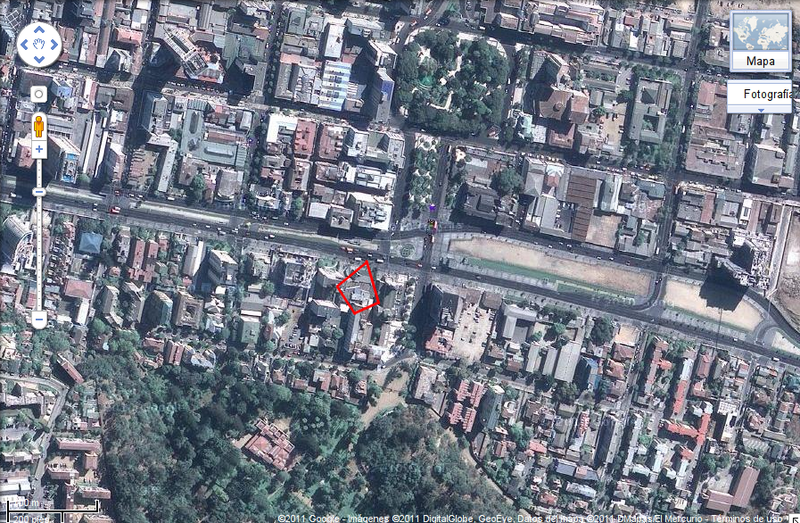
\includegraphics[width=0.7\textwidth]{img/maps.png}
   \caption{Ubicación satelital del lugar}
   \label{fig:mapa}
\end{figure}

{\bf Frontis lugar}

\begin{figure}[h!t]
   \centering
   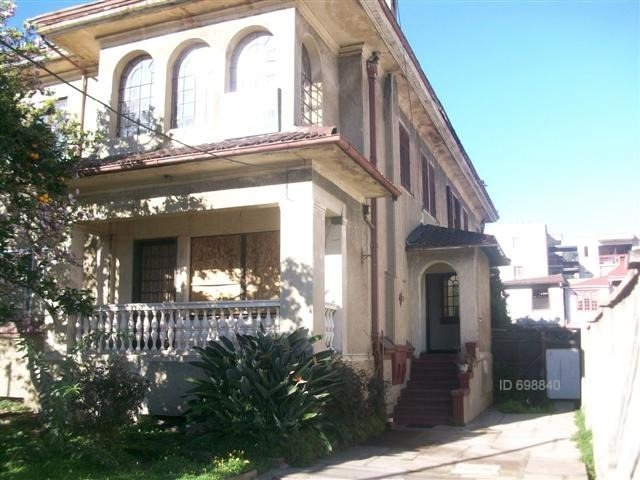
\includegraphics[width=0.7\textwidth]{img/foto_local_1.jpg}
   \caption{Fotografía del frontis del lugar.}
   \label{fig:frontis}
\end{figure}

\newpage
{\bf Propuesta de plano y distribución de lugares}


\begin{figure}[h!t]
   \centering
   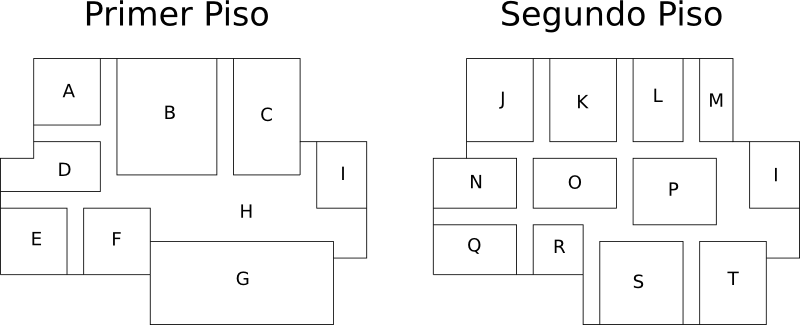
\includegraphics[width=0.8\textwidth]{img/plano.png}
   \caption{Propuesta plano del lugar.}
   \label{fig:plano}
\end{figure}

A continuación se nombran las secciones dentro del lugar establecido
para hacer posible el proyecto \emph{Music Labs}:

\begin{description}
   \item[A:] Baño 1.
   \item[B:] Sala de ensayo 1.
   \item[C:] Comedor
   \item[D:] Baño 2.
   \item[E:] Cocina.
   \item[F:] Sala de reuniones 1.
   \item[G:] Recepción.
   \item[H:] Hall principal.
   \item[I:] Escalera.
   \item[J:] Sala de reuniones 2.
   \item[K:] Espacio Libre (Sala de ensayo 2 a mediano plazo).
   \item[L:] Baño 3.
   \item[M:] Bodega 1.
   \item[N:] Sala de reuniones 3.
   \item[O:] Baño 4.
   \item[P:] Estudio de grabación 1.
   \item[Q:] Salón de eventos.
   \item[R:] Baño 5.
   \item[S:] Espacio Libre (Estudio de grabación 2. a mediano plazo).
   \item[T:] Salón de descanso.
\end{description}

% Cristian
\subsubsection{Obras Físicas}

Para el presente proyecto, se pueden observar tres secciones que están
relacionadas con las obras físicas.

Primero que todo, el arriendo del establecimiento es una obra
fundamental para llevar a cabo el proyecto, el cual puede
ser analizado con detalle en la sección anterior.

Por otro lado, se tienen los costos que van asociados a la adaptación
de ciertos lugares del local para cumplir todas las condiciones iniciales
del proyecto, los que considerarán pequeñas construcciones de obras dentro
del local.

Finalmente, está el costo que conllevará poder adaptar las salas
de grabación y ensayo. No están consideradas en el punto anterior,
por ser un trabajo más especializado, que el retoque de ciertos
lugares del local.


\addtocounter{footnote}{1}
\footnotetext[\value{footnote}]{Valor de la UF al 25 de Mayo del 2011 es de $21,797.19$ CLP}


\begin{table}[h]
\scriptsize
\centering
	\begin{tabular}{|l|r|r|r|r|}
	\hline
	\textbf{Obras físicas}       & \textbf{Cantidad $(m^2)$} & \textbf{Costo por $m^2$ (UF$^{\decimal{footnote}}$)} & \textbf{Costo Total (UF)} & \textbf{Costo Total (CLP)} \\\hline
	Arriendo local (mensual)               & 400                       & 0.115                         & 45.877                   & 1000000     \\\hline
	Adaptaciones necesarias (anual)     & 40                        & 10                            & 400                      & 8718876    \\\hline
	Adaptaciones especializadas (anual) & 15                        & 8                             & 120                      & 2615663     \\\hline
	\textbf{Total}  			 & ---                       & ---                           & 1070.524                 & 23334539   \\\hline
	\end{tabular}
\caption{Descripción Obras Físicas}
\label{tab:obras-fisicas}
\end{table}

La tabla anterior considera que el arriendo se cancelará de forma mensual,
por otro lado las adaptaciones necesarias están consideradas de forma anual,
de la misma forma que las especializadas.

Las adaptaciones necesarias, corresponden a cambios a la estructura
en forma general, las cuales serán necesarias debido a que no es un lugar
nuevo, por lo que al ser una estructura antigua, necesita reparaciones
periódicas.

Las adaptaciones especializadas corresponden a arreglos técnicos en las
salas de ensayo o de grabación.

% Cristian
\subsubsection{Proyectos Complementarios}

No existen proyectos complementarios a ser realizados a corto plazo,
pero si se tiene considerado la posibilidad de encapsular aún más
el macro-servicio que se pretende realizar.

Por lo anteriormente dicho, a mediano plazo se planea tener una flota
de transporte de bandas en la región, y a largo plazo se planea 
tener una tienda especialista en venta de instrumentos de primera
calidad, diferenciándose del resto por la atención personalizada
a cada comprados.

%rfernand
\subsubsection{Calendario de Inversiones}

La inversión inicial del proyecto será distribuida principalmente a lo largo de
los dos primeros meses una vez iniciado el proyecto. En primer lugar se comenzará
por adquirir los diferentes recursos necesarios para el funcionamiento básico
del local. Los meses siguientes se invertirá en la adquisición de los equipos
del estudio de grabación y sala de eventos, las cuales requieren de mayor
programación para su debido uso.

\begin{table}[htb!]
\scalebox{0.8}{
\begin{tabular}{|l|r|r|r|r|r|r|}
\hline
\textbf{Inversión/Periodo}  & \multicolumn{6}{|c|}{\textbf{Año 0}} \\
\hline
 & \textbf{mes 1} & \textbf{mes 2} & \textbf{mes 3}& \textbf{mes 4}& \textbf{mes 5}& \textbf{mes 6}\\
\hline
 %                                              & \       mes 1 &         mes 2  &         mes 3 &         mes 4 &         mes 5 &         mes 6 \\
 Adquisición de Equipos de Sala de Ensayo       & 6.044.794     &              &               &               &               &               \\
 Adquisición de Equipos de Estudio de Grabación &               &    3.523.889 &               &               &               &               \\
 Adquisición de Equipos de Sala de Eventos      &               &              &  6.000.695    &               &               &               \\
 %Adquisición de Software                       &               &              &               &               &               &               \\
 Adquisición equipos de Oficina                 &   665.729     &              &               &               &               &               \\
 Adaptaciones especializadas al Local           & 2.615.663     &              &               &               &               &               \\
 Adaptaciones necesarias al Local               & 8.718.876     &              &               &               &               &               \\
 %Arriendo del Local                             & 1.000.000     &    1.000.000 &  1.000.000    &  1.000.000    &  1.000.000    &  1.000.000    \\
 %Gastos de puesta en marcha                    &               &              &               &               &               &               \\
\hline
\end{tabular}
}
\caption{Calendario de Inversiones. Fuente: Elaboración propia.}
\end{table}

Además, hay que considerar todos los costos mensuales del proyecto, el arriendo
del local\ref{tab:obras-fisicas} y los costos asociados a los sueldos del personal y materias
primas\ref{tab:insumos} utilizadas para la puesta en marcha del mismo.


%jolivaro
\subsubsection{Programa de Reinversiones}

Los equipos utilizados para prestar el servicio
de la empresa tienen en promedio una vida
útil de 6 años, por lo tanto será necesario,
en máximo 6 años, reinvertir para conseguir
equipamiento moderno que permita
mantener la calidad de los servicios prestados.
Obviamente, en la medida que ciertos
equipos presenten problemas será necesario
comprarlos nuevamente, pero esto será una situación
particular a evaluar. En términos generales
al cabo de los 6 años, se hará una gran reinversión
que permitirá a \emph{Music Labs} contar con equipamiento
de última tecnología.

La cantidad de dinero requerida para dicha reinversión
dependerá de los precios de ese momento, pero
no deberían fluctuar más allá del total de
la inversión a realizar en esta etapa.

Además, durante el funcionamiento de la empresa
puede existir la necesidad de expansión, dependiendo
de la demanda y los resultados obtenidos hasta ese 
momento. Las posibilidades de expansión están
dadas por crear nuevas salas de ensayo, estudios de 
grabación y eventos de mayor embergadura. Todo esto
requiere una gran inversión en cuanto a equipamiento
e infraestructura. Además, existe la posibilidad
de abrir una nueva sucursal en Concepción y Santiago, que
fueron los lugares que la macrolocalización determinó
como posibles puntos de funcionamiento del proyecto.
% TO DO
% \red{Y la tabla?}


% Cristian
\subsubsection{Análisis de Materias Primas e Insumos}

Debido a que el presente proyecto corresponde a un servicio
y no a la generación de un producto tangible, la materia prima
será netamente basada en el profesionalismo e intelecto de las
personas que se desarrollen en el proyecto de una forma
profesional y adecuada.

Por otro lado, los insumos directos corresponderán a los elementos 
que se utilicen directamente para el desarrollo de las distintas
actividades dentro del proyecto, es decir, todos los elementos
relacionados a la asesoría musical de bandas emergentes y
de la misma forma, los servicios adicionales ofrecidos.

Finalmente, los insumos indirectos corresponderán a los servicios
básicos, en el caso de \emph{Music Labs}, serán:
\begin{itemize}
	\item Electricidad.
	\item Agua potable.
	\item Telefonía.
	\item Internet.
\end{itemize}

Se especifica en la tabla 13 el detalle de las materias primas
e insumos del proyecto.

\addtocounter{footnote}{1}
\footnotetext[\value{footnote}]{Plan de Minutos ilimitados Movistar}

\addtocounter{footnote}{1}
\footnotetext[\value{footnote}]{Plan Banda Ancha 10 Megas Movistar}

\addtocounter{footnote}{-1}

\begin{table}[h]
\scriptsize
\centering
	\begin{tabular}{|l|r|r|r|r|r|}
	\hline
	\textbf{Materias primas e insumos} & \textbf{Unidades} & \textbf{Cantidad (mensual)} & \textbf{Costo unitario} & \textbf{Costo mensual} & \textbf{Costo Anual} \\\hline
	\blue{Materias Primas} & \multicolumn{5}{|r|}{} \\\hline
	Asesores Informáticos                                       & personas                        & 2                  & 1000000 & 2000000 & 24000000 \\\hline
	Asesores Electrónicos                                       & personas                        & 2                  & 1000000 & 2000000 & 24000000 \\\hline
	Asesores Industriales                                       & personas                        & 1                  & 900000  & 900000  & 10800000 \\\hline
	Asesores Artísticos                                         & personas                        & 1                  & 750000  & 750000  &  9000000 \\\hline
	Asesores Sonidista                                          & personas                        & 2                  & 950000  & 1800000 & 21600000 \\\hline
	\blue{Insumos Directos}                                     & \multicolumn{5}{|r|}{} \\\hline
	Tóner impresora                                             & unidad                          & 1                  & 62990   & 62990   &   755880 \\\hline
	Resma papel                                                 & unidad                          & 5                  & 2700    & 13500   &   162000 \\\hline
	CD's                                                        & unidad                          & 10 (x 50 unidades) & 5690    & 56900   &   682800 \\\hline
	Articulos oficina                                           & unidad                          & 50                 & 1000    & 50000   &   600000 \\\hline
	\blue{Insumos Indirectos}                                   & \multicolumn{5}{|r|}{} \\\hline
	Electricidad                                                & $Kw/h$                          & 400                & 103     & 41200   &   494400\\\hline
	Agua potable                                                & $m^3$                           & 10                 & 1100    & 11000   &   132000 \\\hline
	Telefonía$^{\decimal{footnote}}$ \addtocounter{footnote}{1} & unidad                          & 1                  & 17990   & 17990   &   215880 \\\hline
	Internet$^{\decimal{footnote}}$                             & unidad                          & 1                  & 22990   & 22990   &   275880 \\\hline
	\textbf{Total:}												& ---							  & --- 			   & ---     & 7726570 & 92718840 \\\hline
	\end{tabular}
\caption{Detalle materias primas e insumos}
\label{tab:insumos}
\end{table}

%Javier
\subsubsection{Programas de Trabajo}

Debido a la naturaleza del negocio es necesario
tener personal con distinto tipo de contrato, ya
que hay labores que solamente se requieren en
la medida que exista la demanda por parte
de los clientes. En cambio, otras labores por
ejemplo la realizada por la secretaria, son de
tiempo completo.\\

\textbf{Contrato de tiempo completo}

\begin{itemize}
 \item Secretaria: La labor principal de la secretaria
	será distribuir las horas disponibles de ensayo
	y grabación a las bandas que lo soliciten. Además
	de contactar a los profesionales a cargo de labores
	de asesoría, grabación, ensayo, gestión de eventos, 
	y managers. Además de lo anterior, llevará todas las
	labores comunes de secretaría, relacionadas con la
	naturaleza del negocio.
	
	Su contrato estipulará que la cantidad
	de horas de trabajo serán 8 por día, desde las 09:00
	hasta las 18:00 horas, considerando una hora de colación.
\end{itemize}

\textbf{Contrato a Honorarios}\\

Los trabajadores a continuación serán requeridos en la medida que 
las bandas contraten los distintos servicios ofrecidos.

\begin{itemize}

\item Ingeniero en Sonido: Encargado de la grabación musical, tanto
      en la etapa de grabación, mezcla, masterización y remasterización.
      Además, estará a cargo del sonido en los eventos generados
      por la empresa. La cantidad de Ingenieros en Sonido dependerán
      de la carga de trabajo del momento.

\item Técnico en Sonido: Profesional de nivel técnico encargado
	de la sala de ensayo, permitiendo que las bandas que 
	contraten el servicio puedan utilizar adecuadamente
	la sala. Además, tendrán la labor de apoyar al Ingeniero en Sonido
	en las tareas propias de la grabación musical y amplificación de 
	eventos. La cantidad de Técnicos en Sonido dependerán de la carga 
	de trabajo del momento.

\item Asesor Informático: Empleado de nivel Profesional, de preferencia
      Ingeniero Civil en Informática, encargado de las labores de creación y 
      mantenimiento de páginas Web para las bandas que así lo contraten. Debe
      tener experiencia en Web 2.0 para lograr un eficaz posicionamiento
      de las bandas en la nueva forma en que funciona actualmente la Web.

\item Asesor Musical: Especialista encargado de apoyar a las bandas
      en la etapa de composición, grabación y producción musical.

\item Manager: Especialista con experiencia, encargado de apoyar a las bandas 
      al momento en que busquen sus propios eventos musicales donde presentar
      su trabajo, con el fin de obtener tratos justos y que logren
      beneficiar a las partes interesadas.

\item Publicista: Profesional encargado de la parte creativa relacionada
      con los eventos producidos por la empresa, además de la promoción
      y difusión de las bandas.

\item Contador: A cargo del área de contabilidad y finanzas de la
      empresa.
\end{itemize}

%%%%%%%%

Cabe destacar que los profesionales que se dedican especialmente 
a las bandas (asesores) serán utilizados a medida que sean necesarios, 
por lo que no cuentan con un horario de trabajo determinado, aunque es necesario
notar que, en momentos en que su trabajo sea de corrido, no podrá superar la cantidad
de horas que dictamina el código del trabajo.

Por otro lado, en las salas de ensayo, se trabajará en una modalidad de turno, los cuales
corresponden a:
\begin{itemize}
	\item Turno 1: 09:00 - 18:00, con una hora de colación.
	\item Turno 2: 18:00 - 24:00, con media hora de colación.
\end{itemize}

Estos turnos serán flexibles, en el sentido de que, si la demanda es poca, o prácticamente nula al final 
de uno de los turnos, el encargado de local está facultado para cerrarlo. 

%Marito
\subsubsection{Programa de Producción}

El programa de producción ayudará a determinar la frecuencia con que se presentará 
el servicio. Además, dará una estimación de la cantidad de bandas emergentes
que se podrán atender y asesorar durante un período, en este caso, un año.

Se contempla para este estudio, 1 sala de ensayo, 1 estudio de grabación, 1 salón 
de eventos, además de la asesoría que, como se menciona anteriormente, se realizará
a medida que las bandas soliciten el servicio.

La sala de ensayos se arrienda por 1 (una) hora. Lo que indica que se tendrá alrededor
de 12 horas diarias de disponibilidad, 72 horas a la semana (6 días), 288 horas al mes, y 3456
 horas anuales. En promedio, una banda ensaya entre 2 y 4 horas a la semana, 
por lo que, semanalmente se debe atender alrededor de 18 bandas (se utilizó la cantidad
de horas máxima). Estimando que estas mismas bandas se repetirán de forma semanal, la cantidad
de bandas anuales distintas que pasen por las salas de ensayo no debiera variar de manera significativa
a lo largo de los años, a no ser que, en el futuro, se piense en una ampliación.

El estudio de grabación se arrienda por hora, pero es muy complicado que una banda 
decida estar sólo una hora, pues la grabación de un solo tema, demora bastante más tiempo. 
Entonces, en ese caso, se puede suponer que el uso del estudio de grabación será diario.
Con estas estimaciones, se deberá tener en cuenta que se puede atender a 6 bandas 
semanalmente. Estas agrupaciones no acostumbran grabar todas las semanas, ni todos los meses. 
De hecho, no todas las bandas realizan grabaciones de sus discos, sino que simplemente se 
presentan en locales, por lo que la cantidad de bandas a las cuales se atenderá de forma anual 
debiera ser cercano al mismo número de bandas diferentes que utilizarán las salas de ensayo. 
Cabe destacar que este número sí puede crecer, pues a medida que \emph{Music Labs} se haga 
conocido, sus servicios serán aún más solicitados. Se estima que este crecimiento puede ser 
de 1 banda por cada dos años.

Con respecto a la producción y realización de eventos, se estima que las mismas bandas
que ensayen solicitarán este servicio, al menos una vez en todo el año, pues es la manera
en que mejor se dan a conocer. Si bien, lo ideal es tener todos los fines de semana ocupados 
con esta actividad, se estima que las bandas que utilizarán el servicio, por lo menos la primera 
mitad del primer año, serán las mismas que ensayan y, a medida que \emph{Music Labs} comience
a adquirir un nombre, más bandas solicitarán el servicio de producción y realización de eventos.
Es por esto que se estima que en la segunda mitad del primer año, se pueda aumentar el número
de bandas solicitantes del servicio en alrededor de un 20\%, para luego descender ese crecimiento a 
un 10\%. 

De similar manera se comportará el servicio de posicionamiento web, pues se comenzará a dar
asesoría a una parte de las bandas que utilicen el resto de los servicios, para luego intentar
abarcar un mayor mercado. Ahora bien, este servicio no está ligado directamente con lo musical 
de una banda, por lo que se estima que el número de agrupaciones no superará las 15 en el primer 
año, y el aumento sería de 1 banda por año.

Estos datos se resumen en la siguiente tabla.
\begin{table}[h]
\centering
\footnotesize
	\begin{tabular}{|p{5cm}|c|c|c|c|c|c|c|c|c|c|} \hline
	\backslashbox{\textbf{Servicio}}{\textbf{Año}} & 1 & 2  & 3  & 4  & 5  & 6  & 7  & 8  & 9  & 10 \\ \hline
	Sala de Ensayo                      & 18             & 18 & 18 & 18 & 18 & 18 & 18 & 18 & 18 & 18\\ \hline
	Estudio de Grabación                & 18             & 18 & 19 & 19 & 20 & 20 & 21 & 21 & 22 & 22 \\ \hline
	Producción y realización de eventos & 18             & 21 & 23 & 24 & 25 & 26 & 27 & 28 & 29 & 30 \\ \hline
	Posicionamiento Web                 & 15             & 16 & 17 & 18 & 19 & 20 & 21 & 22 & 23 & 24 \\ \hline
	\end{tabular}
	\caption{Tabla resumen de la cantidad de bandas atendidas por año y por servicio}
\end{table}
%\emph{Music Labs} proveerá sus servicios durante todo el año, pero existen 
%ciertas diferencias en cada una de las actividades.
%
%El servicio de sala de ensayo comenzará cuando una banda solicite las
%instalaciones para poder realizar las prácticas necesarias como grupo musical. 
%Dependiendo de la disponibilidad, se asignará un horario (en común acuerdo con
%la banda) para realizar dicha actividad. Una vez en la sala, se proveerá de los 
%instrumentos necesarios durante el tiempo definido previamente, para que la 
%banda los utilice con libertad, mientras dura su ensayo. Una vez terminado este
%proceso, la banda deja las instalaciones, se revisan los equipos utilizados, y 
%se da el ensayo por finalizado. 
%
%El servicio de grabación, comenzará de forma similar al anterior, con la 
%solicitud de espacio físico y técnicos necesarios para realizar el 
%procedimiento de forma adecuada. Una vez realizada la solicitud, \emph{Music Labs} 
%reserva el espacio por la cantidad de horas definidas por la banda. Este 
%servicio puede incluir la grabación, la mezcla, la postproducción y la 
%masterización. La empresa se preocupará de tener los implementos necesarios
%en el día y hora indicados, para un funcionamiento más fluido. Además, 
%la banda especificará lo que necesita, para no atrasar los procedimientos 
%a seguir.
%
%Con respecto al posicionamiento en las principales redes sociales, el servicio 
%comienza con la solicitud de alguna de las opciones, ya sea página web, 
%cuenta twitter, publicidad, blog, etc. Una vez realizada la solicitud, 
%las personas encargadas realizarán las gestiones necesarias para poder llevar
%a cabo lo solicitado. En el caso de la página web, \emph{Music Labs} se 
%encargará de realizarla, y de buscar el hosting adecuado, además del 
%dominio. Por otro lado, se apoyará también con la asesoría necesaria para
%la utilización de este tipo de servicios.
%
%Para finalizar, con respecto a la producción y realización de eventos, la 
%banda solicitará el servicio y se buscará una fecha adecuada. Este servicio
%se producirá principalmente los fines de semana, pues es el momento en que 
%la mayor cantidad de público puede asistir, lo cual no implica que no se 
%realicen eventos durante la semana, dependiendo de la disponibilidad. Dichos 
%eventos, pueden ser realizados en un salón proporcionado por la empresa, o 
%bien, en algún otro local de la zona, en que existan los contactos (pubs, 
%restaurants, etc). En caso de utilizar las dependencias propias, simplemente
%se ubicará la fecha y hora que acomode, y, posteriormente, se procederá a 
%realizar el evento. En caso de que se decida por otro lugar, \emph{Music Labs}
%hará las gestiones que sean necesarias para que esto se pueda cumplir, de 
%tal manera que los esfuerzos de la banda se concentren principalmente en 
%ensayar su música, y no deban gastar parte de su tiempo buscando la manera de
%darse a conocer. 

\newpage
\subsubsection{Tabla resumen de egresos de la Ingeniería del proyecto}

\begin{table}[htb!]
\centering
%\small
\scriptsize
	\begin{tabular}{|c|c|c|c|c|c|c|c|c|c|c|}

		\hline
		Años & 1 & 2 & 3 & 4 & 5 & 6 & 7 & 8 & 9 & 10\\
		\hline
		Arriendo &  12000 &  12000&  12000&  12000&  12000&  12000&  12000&  12000&  12000&  12000 \\
		\hline
		Equipos de Oficina & 655 & 0&0 &0 &0 & 0 & 367 & 150 &0 & 0\\
		\hline
		Equipos Sala de Ensayo & 6045 & 0 & 0 & 0 & 0 & 0 & 6045 & 0 & 0 & 0 \\
		\hline
		Equipos Grabación & 3524 & 0 & 0 & 0 & 0 & 0  & 3524& 0 & 0 & 0 \\
		\hline
		Equipos Sala de eventos & 6000& 0 & 0 & 0 & 0 & 0 &6000 & 0 & 0 &0 \\
		\hline
		Adaptaciones especializadas & 2616 & 0 & 0 & 0 & 0 & 0 & 0 & 0 & 0 & 0 \\
		\hline
		Adaptaciones necesarias & 8719 & 0 & 0 & 0 & 0 & 0 & 0 & 0 & 0 &0  \\
		\hline
		Materias primas e insumos & 92718 & 92718 & 92718 & 92718 & 92718 & 92718 & 92718 & 92718 & 92718 & 92718 \\
		\hline
		Total anual&  132277 &  104718&  104718&  104718&  104718&  104718& 120649 &  104868&  104718&  104718 \\
		\hline
	\end{tabular}
\caption{Tabla egresos Ingeniería del proyecto (en miles)}
\end{table}
